\chapter{Metodologia}
\label{chap:metodologia}

Este capítulo visa apresentar a metodologia que será empregada na realização desse trabalho, visando atender seus objetivos gerais e específicos.

\section{CARACTERIZAÇÃO DA PESQUISA}
Segundo \citeauthor{wazlawick2014} (\citeyear{wazlawick2014}), a área da Ciência da Computação é normalmente classificada como parte das ciências exatas ou das engenharias, mas diversas subáreas da computação estão mais próximas das ciências sociais. Este trabalho de mestrado irá realizar um estudo de caso, por meio de diagnóstico, documentação e formalização do projeto de extensão CInbora Impactar (\href{https://sigaa.ufpe.br/sigaa/link/public/extensao/visualizacaoAcaoExtensao/1971}{\textit{Link} com detalhes do projeto}), e a realização de práticas de pesquisa-ação em um projeto de Extensão utilizando a Inovação Social Aberta.

As pesquisas científicas, segundo, \citeauthor{wazlawick2014} (\citeyear{wazlawick2014}, pp. 41-42) podem ser classificadas a respeito da sua natureza, como um resumo de assunto, que versa somente sobre a sistematização de uma área de conhecimento, mostrando sua evolução ao longo do tempo, e como se encontra atualmente o estado da arte ou um trabalho original, que apresenta melhorias para teorias existentes ou até mesmo a proposição de novas teorias, para avançar o estado da arte da ciência.

Elas também podem ser classificadas quanto a seus objetivos (\citeauthor{gil2002}, \citeyear{gil2002}, pp. 41-42), como pesquisas exploratórias, descritivas ou explicativas. Na pesquisa exploratória o autor irá examinar uma série de fenômenos e variáveis buscando maior familiaridade com o problema, tornando-o mais concreto, e criando hipóteses acerca deste. Já na descritiva os fatos serão abordados como o são, através da descrição das características do objeto a ser estudado. E a pesquisa explicativa, além de analisar os dados, irá buscar responder às causas desses dados e suas explicações.

Uma terceira classificação trazida por \citeauthor{wazlawick2014} (\citeyear{wazlawick2014}, pp. 21-24) versa acerca dos procedimentos técnicos que serão realizados na pesquisa, que podem ser classificados por Pesquisa bibliográfica, documental, experimental, de levantamento ou pesquisa-ação. A pesquisa bibliográfica é um dos primeiros passos e visa o estudo de materiais científicos que já foram publicados anteriormente a respeito de determinado tema. Já a pesquisa documental analisa documentos, relatórios, normas, bancos de dados, e outros, que não estão disponíveis de forma sistematizada. A pesquisa experimental realiza tentativas experimentais através da manipulação de variáveis e/ou fatores por parte do pesquisador para observar os resultados dos mesmos. A pesquisa de levantamento busca dados a respeito do ambiente, de comportamentos, das pessoas inseridas nele, por meio de questionários, \textit{surveys}, e afins. E na pesquisa-ação o pesquisador interage diretamente com aqueles que estão sendo os objetos da pesquisa, visando promover mudanças e geração de conhecimento, unindo assim, a prática com a teoria.

\citeauthor{creswell2007} (\citeyear{creswell2007}, p. 27) traz também três métodos de pesquisa, sendo conjuntos de procedimentos a serem adotados para coleta, análise e interpretação de dados, e são os métodos quantitativos, qualitativos e mistos. Nos métodos quantitativos o pesquisador utiliza de estratégias e técnicas de pesquisa como levantamento e experimentos para gerar dados estatísticos que permitam sua observação e mensuração Os métodos qualitativos utilizam de estratégias mais voltadas para a observação de comportamento e do ponto de vista dos participantes da pesquisa sobre os fenômenos estudados, por meio de fenomenologia, etnografia, estudo de casos, e outros. E os métodos mistos empregam o uso das duas abordagens em conjunto.

Essa proposta de trabalho classifica-se como:

\begin{quadro}[H]
\caption{Classificação metodológica da proposta de trabalho}
\centering
\begin{tabular}{|
>{\columncolor[HTML]{9B9B9B}}l |l|}
\hline
\textbf{Método de Pesquisa}      & Pesquisa Qualitativa                                                                                                \\ \hline
\textbf{Natureza}      & Trabalho Original                                                                                                             \\ \hline
\textbf{Objetivos}     & Exploratório e descritivo                                                                                                     \\ \hline
\textbf{Procedimentos} & \begin{tabular}[c]{@{}l@{}}Revisão rápida de literatura, \\estudo de caso e pesquisa-ação.\end{tabular} \\ \hline
\end{tabular}
\vspace{0.2cm}

{\centering Fonte: O autor (2024). \par}
\end{quadro}

\section{DESENHO DA PESQUISA}
\label{desenhodepesquisa}

Segundo \citeauthor{marconi2003} (\citeyear{marconi2003}), o desenvolvimento de um projeto de pesquisa compreende seis passos: 
“Seleção do tópico ou problema para a investigação, definição e diferenciação do problema, levantamento de hipóteses de trabalho, coleta, sistematização e classificação dos dados, análise e interpretação dos dados e relatório do resultado da pesquisa”.

Esses passos podem ser agrupados em quatro fases: preparação de pesquisa, fases da pesquisa, execução da pesquisa e relatório de pesquisa. A preparação de pesquisa será desconsiderada aqui, por envolver escolha do tema, constituição de equipe de trabalho, cronograma e outros. \cite{marconi2003}


Na etapa de Fases da pesquisa, serão tratados: a escolha do problema que será investigado, a definição deste, e o levantamento das hipóteses acerca do problema. Essa etapa irá envolver:
\begin{itemize}
    \item \textbf{Revisão rápida de literatura}: visa observar o atual panorama da inovação social aberta praticada pelas universidades em instituições do terceiro setor nas principais bases de dados da área da ciência da computação, através da metodologia de revisão rápida proposta por \citeauthor{cartaxo2020} (\citeyear{cartaxo2020});
    \item \textbf{Identificação dos principais atores:} como a inovação social aberta envolve diferentes instituições, e por consequência, uma gama de diferentes atores, deverão ser identificados quais os principais que deverão ser observados com uma maior atenção, e que poderão proporcionar \textit{feedbacks} posteriores a equipe de pesquisa sobre os métodos propostos.
    \item \textbf{Criação do protocolo de entrevistas, grupos focais e formulários}: para colher os \textit{feedbacks} dos principais atores envolvidos, serão criadas estratégias de entrevistas, grupos focais e formulários com os participantes. Essas entrevistas deverão ser validadas anteriormente pela equipe de pesquisa, antes de serem aplicadas.
\end{itemize}

Na etapa de Execução da pesquisa será realizada a coleta e análise de dados, a criação do processo e validação, que envolverá: 
\begin{itemize}
    \item \textbf{Realização das entrevistas, grupos focais e formulários:} realização do que foi concebido na etapa anterior;
    \item \textbf{Análise das entrevistas, grupos focais e formulários}: serão analisadas as entrevistas, grupos focais e formulários, além de todas as questões colocadas pelos entrevistados;
    \item \textbf{Criação do processo para projeto de extensão}: a criação do projeto de Extensão utilizando a Inovação Social Aberta no terceiro setor, após observar os \textit{feedbacks} colhidos nas entrevistas;
    \item \textbf{Validação do processo para projeto de extensão}: o processo proposto será validado durante sua execução, e os \textit{feedbacks} serão coletados durante a análise de dados, que podem ocorrer diversas vezes.
\end{itemize}

A etapa de Relatório de pesquisa trará os resultados obtidos através da pesquisa, suas conclusões e metodologia utilizada. Essa última etapa é a publicização do que foi realizado em toda a pesquisa, e consiste em:
\begin{itemize}
    \item \textbf{Sintetização dos resultados obtidos}: A exposição de todo o conhecimento obtido com os dados trabalhados durante a pesquisa;
    \item \textbf{Confecção da Dissertação}: Escrita da dissertação de mestrado;
    \item \textbf{Apresentação do trabalho}: Apresentar uma sumarização de toda a pesquisa para a banca;
    \item \textbf{Correções finais}: realizar correções na dissertação conforme as orientações da banca.
\end{itemize}

A pesquisa será realizada em ciclos iterativos, visando o incremento das sugestões de melhorias propostas pelos \textit{stakeholders} no processo ao longo da sua execução. Por conta disso, algumas etapas serão provavelmente realizadas mais de uma vez. Esses passos são necessários para garantir o procedimento e o tratamento científico exigido pelo trabalho. Para facilitar a compreensão da forma como a pesquisa se desenvolverá, a figura abaixo traz uma síntese do desenho da pesquisa:

\begin{figure}[H]
    \caption{Desenho de pesquisa proposto}
    \centering
    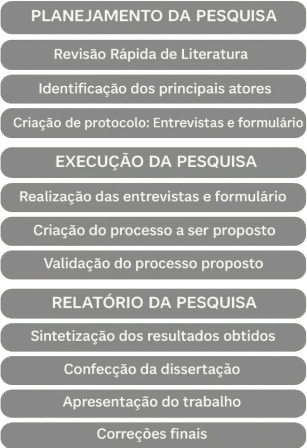
\includegraphics[width=0.6\linewidth]{images/metodologia/desenhodepesquisa.png}
    \label{fig:desenhodepesquisa}
    \vspace{0.2cm}

{\centering Fonte: O autor (2024), baseado em Marconi e Lakatos (2003). \par}
\end{figure}



\section{Plano de Pesquisa-Ação}
\label{pesquisaacao}

Segundo \citeauthor{tripp2005} (\citeyear{tripp2005}), a pesquisa-ação é uma forma de investigação-ação que utiliza as técnicas já consagradas da pesquisa científica por meio de ações tomadas para a melhoria da prática. Possui as fases de: Planejamento, implementação e avaliação, e essas fases ocorrem tanto para a parte da pesquisa (teórica) quanto a parte da ação (prática), e serão produzidos dados sobre os efeitos ocorridos advindos das mudanças empregadas.

A pesquisa-ação a ser realizada possuirá como universo o projeto de extensão CInbora Impactar, coordenador pelo Professor Kiev Gama. Esse projeto é uma iniciativa que visa promover a interação entre a \gls{UFPE} e a comunidade por meio da colaboração com o Projeto Bora Impactar \url{https://www.instagram.com/boraimpactarrecife/}, da Secretaria de Ciência, Tecnologia e Inovação da Prefeitura do Recife, possibilitando o desenvolvimento de soluções de software que atendam às necessidades de \gls{ONG}s do Recife, e também o projeto de extensão CInovação Social, coordenado pelo estudante Pedro Rodolfo e pelo Professor Kiev Gama, em parceria com a ONG Gris Social \url{https://www.instagram.com/gris.solidario/}, que busca a promoção da interação entre a \gls{UFPE} e o terceiro setor, de uma forma direta, não possuindo um intermediário como o projeto CInbora Impactar, visando uma relação dialógica, de troca de saberes.

\par\vspace{1\baselineskip}

\begin{figure}[H]
    \caption{Partes envolvidas}
    \centering
    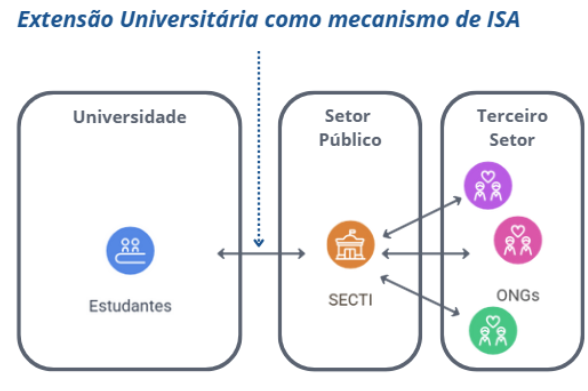
\includegraphics[width=0.6\linewidth]{images/metodologia/partesenvolvidas.png}
    \label{fig:partesenvolvidas}
    \vspace{0.2cm}

{\centering Fonte: O autor (2025). \par}
\end{figure}

Baseado no ciclo de pesquisa-ação de \citeauthor{staron2020} (\citeyear{staron2020}), o plano de pesquisa-ação, proposto nesse trabalho, constitui-se de 5 fases num período de 5 meses, como mostrado na imagem abaixo:

\begin{figure}[H]
    \caption{Ciclo de pesquisa-ação}
    \centering
    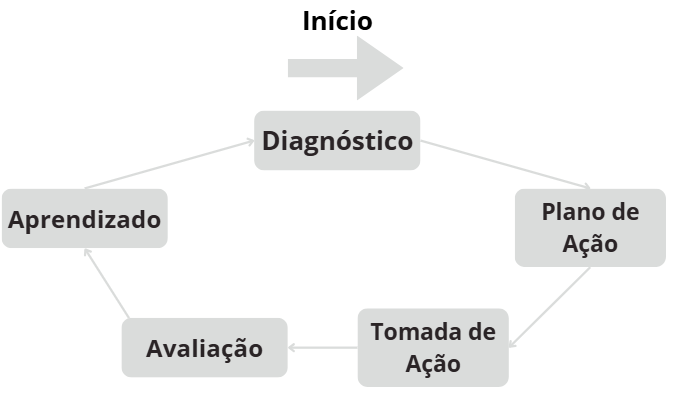
\includegraphics[width=0.5\linewidth]{images/metodologia/pesquisaacao.png}
    \label{fig:pesquisaacao}
    
    Fonte: Adaptado de \citeauthor{staron2020} (\citeyear{staron2020}, p. 3).
\end{figure}


\textbf{1. Diagnóstico — 4 semanas de duração}

Nessa seção, o atual planejamento e metodologias de execução do projeto por parte do professor serão analisados, além de uma identificação inicial das oportunidades de melhoria, focando na interação maior entre os envolvidos, possibilitando um maior processo de inovação aberta. 
Ações: 
\begin{itemize}
\item Realização de entrevistas com os estudantes e o professor acerca do que é esperado para o projeto, sua execução e seus resultados. 
\par\vspace{1\baselineskip}

\end{itemize}

\textbf{2. Plano de ação — 4 semanas de duração}

Será realizado um plano de projeto de Extensão, utilizando práticas já existentes de Inovação Social Aberta. 
Ações:
\begin{itemize}
    \item Levantamento de atores envolvidos;
    \item Criação de proposta de atividades para promover a colaboração entre os atores;
    \item Criação de cronograma proposto para intervenção.
\par\vspace{1\baselineskip}

\end{itemize}

\textbf{3. Tomada de ação —  4 semanas de duração}

Essa fase irá ser executada em uma interação mais direta com o professor e os estudantes, enquanto os mesmos estão trabalhando no processo de construção do artefato que será apresentado posteriormente. Ações:
\begin{itemize}
    \item Monitoramento do impacto sobre os \textit{stakeholders} envolvidos a respeito da execução do projeto
\par\vspace{1\baselineskip}

\end{itemize}

\textbf{4. Avaliação — 4 semanas de duração}

Essa etapa irá verificar se de fato as ações propostas causaram algum impacto sobre os atores envolvidos, e também nos artefatos produzidos pelos estudantes. Ações:
\begin{itemize}
    \item Análise do processo de pesquisa-ação até o momento;
    \item Análise dos artefatos produzidos pelos estudantes;
    \item Grupos focais e formulários com os envolvidos, sobre o processo de interação e colaboração entre os envolvidos;
    \item Identificação de possíveis melhorias.
\par\vspace{1\baselineskip}

\end{itemize}

\textbf{5. Aprendizado — 4 semanas de duração}

Nessa última fase será documentado todo o aprendizado obtido ao longo da execução da pesquisa-ação, e construção do possível processo a ser proposto. Ações:
\begin{itemize}
    \item Documentação das lições aprendidas;
    \item Documentação dos possíveis pontos de melhoria;
    \item Documentação dos impactos sobre todos os envolvidos e sobre o projeto.
\end{itemize}



\section{Análise de Dados}
\label{analisededados}

A análise dos dados será realizado através dos seguintes passos:

\begin{itemize}
    \item \textbf{Transcrição}: Todas as entrevistas e grupos focais serão transcritos por meio de Inteligência Artificial, e serão posteriormente revisadas pelos pesquisadores, a fim de garantir fidelidade à fala dos participantes.
    \item \textbf{Organização dos dados:} Atribuição das falas a cada um dos entrevistados e posterior anonimização das falas, substituindo nomes por pseudônimos ou códigos e armazenamento seguro dos dados obtidos, e organização separada dos grupos focais e entrevistas. Em segunda execução, foi realizada análise de dados de entrevistas e grupos focais com os estudantes e colaboradores da ONG que foi aplicado o projeto de extensão. 
    \item \textbf{Análise de Conteúdo:} Será aplicada a Análise de Conteúdo de acordo com \citeauthor{bardin2011} (\citeyear{bardin2011}):
	\begin{itemize}
	    \item \textbf{Pré-análise:} Identificação das categorias consoante as falas dos participantes;
	\item \textbf{Exploração do material:} Codificação, classificação e agregação para agrupamento de falas com temas semelhantes para identificar possíveis padrões, por meio de ferramentas de análise;
	\item \textbf{Tratamento dos resultados:} inferência e interpretação dos dados obtidos e tratados.
	\end{itemize}


\end{itemize}

\subsection{Aspectos Éticos}
O projeto de pesquisa foi aprovado no Comitê de Ética em Pesquisa da \gls{UFPE}, com o Certificado de Apresentação de Apreciação Ética de n.º 87185225.7.0000.5208, contendo detalhes da Metodologia, Métodos de Recrutamento de Participantes, Critérios de Inclusão e Exclusão, Riscos e mitigação, dentre outras informações pertinentes. Todos os participantes da pesquisa assinaram um Termo de Consentimento Livre e Esclarecido. O modelo deste termo encontra-se no Apêndice B. Os demais Termos utilizados possuem apenas mudanças pontuais conforme o perfil dos participantes (Estudantes, profissionais da prefeitura e colaboradores da ONG), além do termo do formulário \textit{online}.

\subsection{Produto final}

Como produto técnico deste presente mestrado profissional, será desenvolvido um Guia básico de boas práticas para a aplicação da Inovação Social Aberta (ISA) em projetos de Extensão Universitária, a partir da sistematização dos dados obtidos durante o ciclo de pesquisa-ação, nos projetos CInbora Impactar e CInovação Social. Nestes projetos, serão analisados tanto a percepção dos estudantes quanto dos envolvidos das instituições parceiras, sobre sua vivência no projeto, os acertos e desafios metodológicos, estratégias de engajamento, e comunicação entre universidade e instituições parceiras.

Esse guia é destinado a docentes, discentes e gestores de organizações do terceiro setor, e visa fornecer orientações práticas, replicáveis e adaptáveis para equipes extensionistas que possuem interesse na implementação de ações colaborativas e dialógicas no campo da Inovação Social Aberta, voltada para a concepção de artefatos digitais como meio de transformação social.

\section{PROJETO DE EXTENSÃO CINOVAÇÃO SOCIAL}
\label{cinovacaosocial}

O projeto CInovação Social foi concebido visando a prática da Inovação Social Aberta por meio da Extensão Universitária, voltado para estudantes do curso de Sistemas de Informação do \gls{CIn}/\gls{UFPE}, em parceria com uma \gls{ONG}, no caso de sua primeira execução, com a GRIS Solidário.

A organização se situa no bairro da Várzea, e o seu cerne é o atendimento e apoio lúdico-pedagógico para crianças em situação de vulnerabilidade social e também às suas mães, porém também possui uma forte atuação em pautas acerca de conscientização e enfrentamento ao racismo ambiental.

A escolha de atuação com uma \gls{ONG} se deu ao fato do dado apontado por Gama, que relata que ONGs possuem poucos recursos humanos e financeiros para executarem exitosamente suas atividades inovativas. E a escolha em particular da GRIS Solidária se deu em decorrência de sua proximidade com a \gls{UFPE}, visando facilitar a vivência dos espaços da ONG presencialmente pelos estudantes que irão atuar no projeto de extensão.

Apesar de ser um projeto voltado para a concepção de artefatos digitais por meio da computação, o principal foco do projeto versa sobre as pessoas que estão envolvidas nele, e todo o impacto que pode ser gerado pela relação dialógica entre os estudantes e a sociedade.

A metodologia vivenciada no projeto é uma adaptação da \textit{Speedplay} de Maria Ângela Ferrario, que preconiza a concepção de artefatos digitais como veículos de mudança social. É voltada para comunidades que possuem um difícil acesso pelo poder público e que necessitem de soluções que sejam realizadas num espaço de tempo reduzido, dispondo de metodologias ágeis para essa finalidade.

No caso do CInovação Social, o artefato digital construído foi uma Aplicação \textit{Web}, que pode ser utilizada pela ONG tanto por computadores quanto por dispositivos móveis, como solicitado pela própria organização, em decorrência de nem todos os seus colaboradores possuírem acesso fácil a computadores de mesa.

Junto a metodologia \textit{Speedplay} foi adotado o \textit{Vibecoding}, ou programação via \gls{IA}, na qual os estudantes utilizaram algumas ferramentas para gerar as páginas que compõe o núcleo do projeto, e ao longo do desenvolvimento foram incrementando via programação tradicional novas funcionalidades e detalhes ao artefato digital. A utilização de \gls{IA} visa gerar no projeto uma cultura de curadoria de soluções, não apenas programação, levando os esforços dos seus participantes para um maior foco em lógica e propósito da equipe.

Apesar do desenvolvimento ser realizado em conjunto com tecnologias de \gls{IA}, durante o projeto foi amplamente ressaltada a importância da utilização destas tecnologias de forma responsável, através das seguintes orientações:
\begin{itemize}
    \item Revisão do código gerado;
    \item Utilização de \gls{IA} de forma ética;
    \item Combinação do uso de \gls{IA} com boas práticas de engenharia de software;
    \item Documentação das decisões tomadas;
    \item Uso da \gls{IA} como apoio, não como substituto do pensamento.
\end{itemize}

A dinâmica do projeto se deu através da execução de cada \textit{“mini-sprint”} resultando em um pequeno protótipo a ser incrementado nas posteriores \textit{sprints}. O início do projeto deu-se via um momento de vivência dos estudantes nos espaços físicos da \gls{ONG}, que foi chamado no projeto de \textit{Ideathon}, baseado na etapa do \textit{Speedplay}, que Maria Ângela Ferrario chama de Ponto focal, que é um momento de co-criação de projeto de protótipo. No caso do CInovação Social, o \textit{Ideathon} resultou num \textit{wireframe} co-criado com a \gls{ONG}.

\begin{figure}[H]
    \caption{Estudantes co-criando com a ONG}
    \centering
    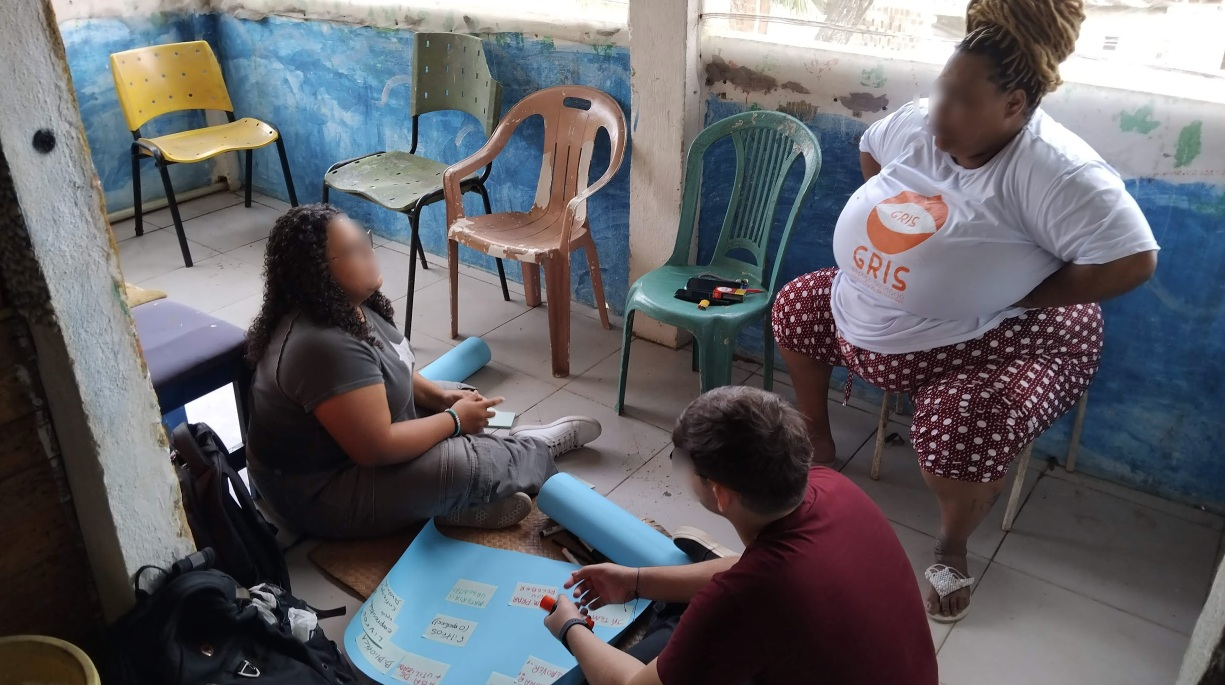
\includegraphics[width=0.6\linewidth]{images/metodologia/ong001.jpeg}
    \label{fig:ong001}
    \vspace{0.2cm}

{\centering Fonte: O autor (2025). \par}
\end{figure}

\begin{figure}[H]
    \caption{Estudantes realizando prototipação via \textit{Wireframe}}
    \centering
    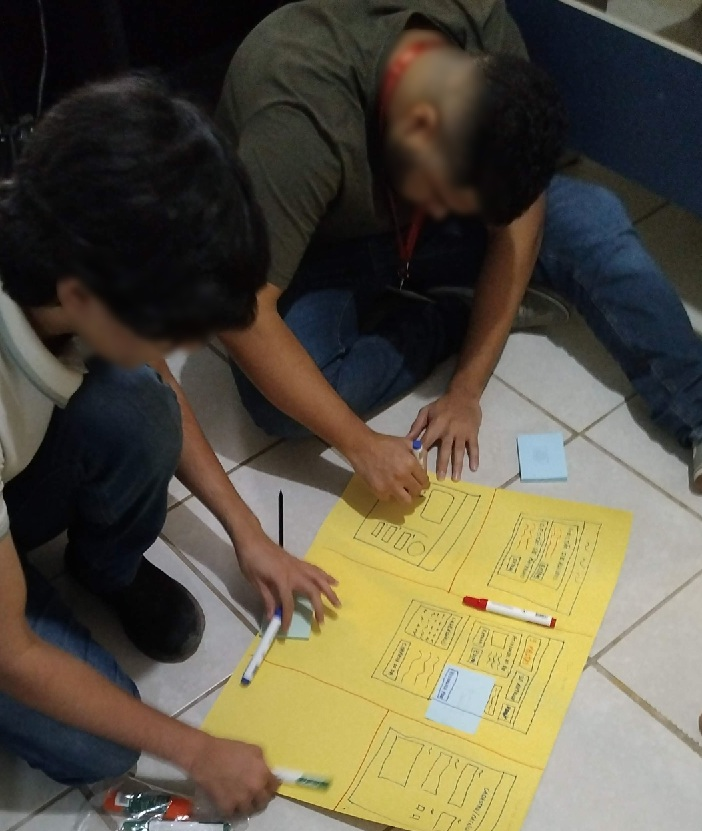
\includegraphics[width=0.6\linewidth]{images/metodologia/ong002.jpeg}
    \label{fig:ong002}
    \vspace{0.2cm}

{\centering Fonte: O autor (2025). \par}
\end{figure}


O cronograma do projeto foi o seguinte, dentro dos quatro ciclos do Speedplay:
\par\vspace{1\baselineskip}

\textbf{Ciclo 1 (Experimentação inicial)}
    \begin{itemize}
        \item Dia 17/08 –\textit{ Prompt-base}
        \item Dia 18 à 20/08 – \textit{Sprint} 1 - Início do \gls{MVP}
        \item Dia 21/08 – \textit{Sprint Review}  - Analisar primeira versão do \gls{MVP} e ajuste do \textit{backlog};
    \end{itemize}
\par\vspace{1\baselineskip}

\textbf{Ciclo 2 (Aprimoramento)}
    \begin{itemize}
        \item Dia 22/08 à 24/08 - \textit{Sprint} 2  - Refinar \gls{MVP} e aplicar as melhorias apontadas na última \textit{Sprint Review}
        \item Dia 25/08 - \textit{Sprint Review} - Verificar a aplicação das melhorias realizadas
        \item Dia 26/08 à 28/08 - \textit{Sprint} 3 - Refinamento do \gls{MVP} e adição de funcionalidades
        \item Dia 29/08 - \textit{Status Report} 1 - Verificação de atendimento de requisitos com \gls{ONG}
    \end{itemize}
\par\vspace{1\baselineskip}

\textbf{Ciclo 3 (Validação e Iteração)}
    \begin{itemize}
        \item Dia 30/08 à 01/09 - \textit{Sprint} 4 - Refinamento do \gls{MVP} e adição de funcionalidades
        \item Dia 02/09 - \textit{Sprint Review} - \textit{Feedback} acerca do \gls{MVP}
        \item Dia 03/09 à 05/09 - \textit{Sprint} 5 - Ajustes e incrementos finais
        \item Dia 06/09 - \textit{Status Report} 2 - Validação do \gls{MVP}
    \end{itemize}
\par\vspace{1\baselineskip}

\textbf{Ciclo 4 (Fechamento e Entrega)}
    \begin{itemize}
        \item Dia 07/09 à 09/09 - \textit{Sprint} 6 - Finalização do \gls{MVP} e preparação para apresentação final
        \item Dia 10/09 - \textit{Sprint Review} - Verificação de últimos ajustes finos e correções na interface
        \item Dia 11/09 à 12/09 - \textit{Sprint} final - Ajustes verificados na última SR
        \item Dia 13/09 - Apresentação final no Espaço \textit{Pitch} - \gls{CIn}/\gls{UFPE}
    \end{itemize}

O projeto contou com a participação direta de seis estudantes do curso de Sistemas de Informação, como equipe responsável pelo desenvolvimento do artefato digital, duas colaboradoras da GRIS Solidário como fonte de informação, participantes da co-criação e validação, o professor orientador auxiliando no processo metodológico e dois pesquisadores na coordenação, coordenando o processo extensionista, e realizando mentoria com os estudantes e alinhamentos necessários com a \gls{ONG}.

Apesar das datas programadas, algumas vezes, a \gls{ONG} teve uma dificuldade em manter as datas agendadas, por conta de adversidades, um quantitativo reduzido de voluntários, onde a própria coordenadora da \gls{ONG} se desdobrou diversas vezes para executar diversas tarefas diferentes na instituição.
